Le diagramme de cas d'utilisation permet de d\'{e}crire l'interaction entre
l'acteur et le syst\`{e}me.
Le cas d'utilisation est une description des interactions qui vont permettre \`{a}
l'acteur d'atteindre son objectif en utilisant le syst\`{e}me. Un acteur et un cas
d'utilisation sont mis en relation par une association repr\'{e}sent\'{e}e par une
ligne.
Le but principal du diagramme du cas d'utilisation est de d\'{e}finir le syst\`{e}me
du point de vue des utilisateurs et de d\'{e}finir les limites pr\'{e}cises du syst\`{e}me en
utilisant une notation tr\`{e}s simple






\FloatBarrier
\begin{figure}[H]
\center
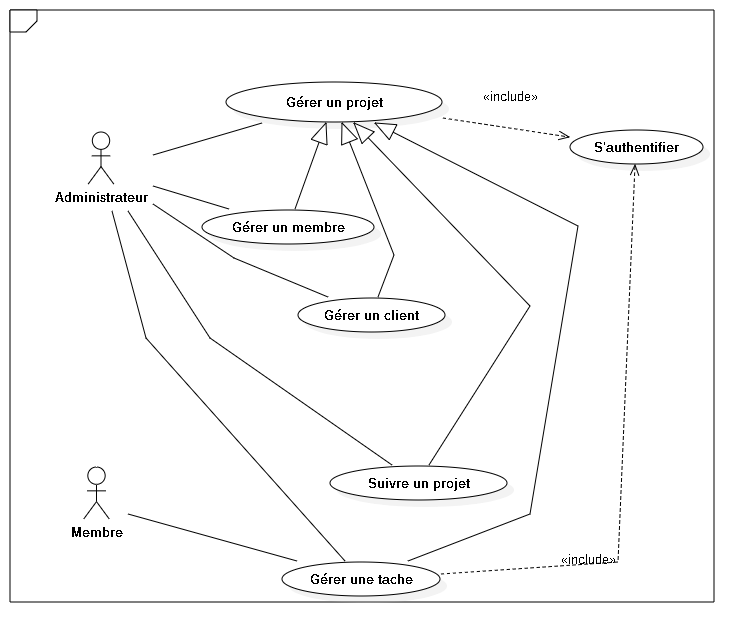
\includegraphics[width=13cm,height=16cm]{./figures/ucG.png}
\caption{Diagramme de cas d'utilisation g\'{e}n\'{e}rale.}

\end{figure}
\FloatBarrier 